%%%%%%%%%%%%%%%%%%%%%%%%%%%%%%%%%%%%%%%%%%%%%%%%%%%%%%%%%%%%%%%%%%%%%%
% This layout was adapted from one found at latextemplates.com which
% was adapted from another.
%
% License: CC BY-NC-SA 3.0
% (http://creativecommons.org/licenses/by-nc-sa/3.0/)
%
% Original header:
%
% This is a LaTeX version of the sample laboratory report from
% Virginia Tech's copyrighted 08-09 CHEM 1045/1046 lab manual.
% Reproduction of this one appendix section for academic purposes
% should fall under fair use.
%
%%%%%%%%%%%%%%%%%%%%%%%%%%%%%%%%%%%%%%%%%%%%%%%%%%%%%%%%%%%%%%%%%%%%%%

\documentclass{article}

\usepackage{graphicx}
%\usepackage[acronym]{glossaries} % Lets us use acronyms
\usepackage{multicol}
\usepackage{amsmath}
\usepackage{siunitx} % SI units in math mode
\usepackage{subcaption}

\author{}
\title{ELEC-313 \\ Lab 3: Diode Circuits\\ }
\date{\today}

%\loadglsentries{acronyms} % Actually loads 'acronyms.tex'
%\makeglossaries

\begin{document}

\maketitle

\begin{center}
  \begin{tabular}{lr}
    Date Performed: & September 25, 2013 \\
    Partners: & Charles Pittman \\
    & Stephen Wilson \\
  \end{tabular}
\end{center}

\newpage

\tableofcontents
\listoffigures
\listoftables

\newpage

% Number the enumerate environment (unordered lists) by letter:
\renewcommand{\labelenumi}{\alph{enumi}.}

\section{Objective}
\label{sec:objective}

The objective is to construct, measure, and observe the behavior of two common diode circuits: a voltage rectifier, and a voltage regulator.

\section{Equipment}
\label{sec:equipment}

\begin{tabular}{ll}
  \centering
  Diode: 1N4007 & Power supply: HP E3631A \\
  Zener diode: 1N5231 & Function generator: HP 33120A \\
  Resistors: \SI{47}{\ohm} & Multimeter: Fluke 8010A \\
  Capacitor: \SI{1}{\micro\farad} & Oscilloscope: Agilent 54622D \\
  Resistive decade box: HeathKit IN-3117 \\
\end{tabular}

\section{Schematics}
\label{sec:schematics}

\begin{figure}[hbtp]
  \centering
  \begin{subfigure}[b]{0.6\textwidth}
    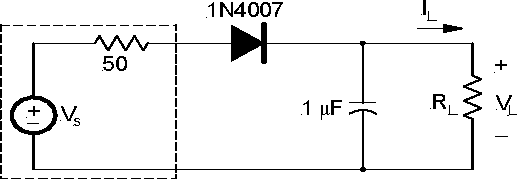
\includegraphics[width=\textwidth]{volt_rect}
    \caption{\label{fig:volt_rect} Voltage rectifier circuit.}
  \end{subfigure}%
  ~
  \begin{subfigure}[b]{0.4\textwidth}
    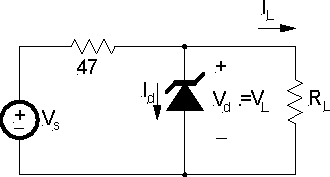
\includegraphics[width=\textwidth]{volt_reg}
    \caption{\label{fig:volt_reg} Voltage regulator circuit.}
  \end{subfigure}
  \caption{\label{fig:circuits_tested} Circuits used in this lab.}
\end{figure}

\section{Procedure}
\label{sec:procedure}

\subsection{Rectifier}
\label{sec:rectifier}

% The circuit in Figure~\ref{fig:circuit1} was constructed with $R =
% \SI{470}{\ohm}$ and the power supply as $V_s$.  The actual resistance
% was measured with one a multimeter and recorded in
% Table~\ref{tab:percent_diff} along with the percent difference calculated
% (Eq~\ref{eq:percent_diff}).  Next, the multimeters were used to
% measure voltage across and current through the diode ($V_d$ and $I_d$,
% respectively) while $V_s$ was swept from \SI{-5}{V} to \SI{+10}{V}.
% The step size from \SI{-5}{V} to \SI{0}{V} and from \SI{5}{V} to
% \SI{10}{V} was \SI{0.5}{V}, and \SI{0.25}{V} from \SI{0}{V} to
% \SI{5}{V}.  These values were recorded in Table~\ref{tab:part_a} and
% plotted in Figure~\ref{fig:combined_graph}.

\subsection{Voltage Regulator}
\label{sec:volt_reg}

% The circuit in Figure~\ref{fig:circuit1} was constructed with the
% resistive decade box as $R$ and the power supply as $V_s$.  The
% multimeters were again used to measure diode voltage ($V_d$) and
% current ($I_d$).  This time $V_s$ was held at \SI{10}{V} and $R$
% varied: \SI{200}{\ohm}, \SI{500}{\ohm}, \SI{1}{\kilo\ohm},
% \SI{2}{\kilo\ohm}, \SI{5}{\kilo\ohm}, \SI{10}{\kilo\ohm},
% \SI{20}{\kilo\ohm}, \SI{50}{\kilo\ohm}, \SI{100}{\kilo\ohm}.  These
% values were recorded in Table~\ref{tab:part_b} and plotted in
% Figure~\ref{fig:combined_graph}.

\section{Results}
\label{sec:results}

\begin{table}[hbtp]
  \centering
  \begin{tabular}{ccc}
    Nominal & Measured & Difference \\
    (\si{\micro\farad}) & (\si{\micro\farad}) & \\
    \hline
    1 & 0.938 & 6.2\% \\
  \end{tabular}
  \caption{\label{tab:cap} Percent difference of capacitor in rectifier circuit.}
\end{table}

\begin{table}[hbtp]
  \centering
  \begin{tabular}{cccccc}
    $V_S$ & $V_{max}$ & $V_{min}$ & $V_r$ & $V_{DC}$ & Ripple \\
    (\si{V_{peak}}) & (\si{V}) & (\si{V}) & (\si{V}) & (\si{V}) & \\
    \hline
    1 & 0.488 & 0.369 & 0.119 & 0.429 & 24.4\% \\
    2 & 1.41 & 1.10 & 0.310 & 1.26 & 22.0\% \\
    3 & 2.39 & 1.88 & 0.510 & 2.14 & 21.3\% \\
    4 & 3.31 & 2.38 & 0.930 & 2.85 & 28.1\% \\
    5 & 4.25 & 3.19 & 1.06 & 3.72 & 24.9\% \\
  \end{tabular}
  \caption{\label{tab:rect_vp_vdc} AC input vs. DC output of rectifier circuit, where $R_L=\SI{10}{\kilo\ohm}$.}
\end{table}

\begin{table}[hbtp]
  \centering
  \begin{tabular}{cccccc}
    $R_L$ & $V_{max}$ & $V_{min}$ & $V_r$ & $V_{DC}$ & Ripple \\
    (\si{\ohm}) & (\si{V}) & (\si{V}) & (\si{V}) & (\si{V}) & \\
    \hline
    1k & 4.13 & 0.440 & 3.69 & 2.29 & 89.3\% \\
    10k & 4.25 & 3.19 & 1.06 & 3.72 & 24.9\% \\
    100k & 4.321 & 4.193 & 0.128 & 4.257 & 2.962\% \\
  \end{tabular}
  \caption{\label{tab:load_v_ripple} Effect of $R_L$ on DC output in rectifier circuit.}
\end{table}

\begin{figure}[hbtp]
  \centering
  % GNUPLOT: LaTeX picture
\setlength{\unitlength}{0.240900pt}
\ifx\plotpoint\undefined\newsavebox{\plotpoint}\fi
\sbox{\plotpoint}{\rule[-0.200pt]{0.400pt}{0.400pt}}%
\begin{picture}(1500,900)(0,0)
\sbox{\plotpoint}{\rule[-0.200pt]{0.400pt}{0.400pt}}%
\put(171.0,131.0){\rule[-0.200pt]{4.818pt}{0.400pt}}
\put(151,131){\makebox(0,0)[r]{ 0}}
\put(1419.0,131.0){\rule[-0.200pt]{4.818pt}{0.400pt}}
\put(171.0,212.0){\rule[-0.200pt]{4.818pt}{0.400pt}}
\put(151,212){\makebox(0,0)[r]{ 0.5}}
\put(1419.0,212.0){\rule[-0.200pt]{4.818pt}{0.400pt}}
\put(171.0,292.0){\rule[-0.200pt]{4.818pt}{0.400pt}}
\put(151,292){\makebox(0,0)[r]{ 1}}
\put(1419.0,292.0){\rule[-0.200pt]{4.818pt}{0.400pt}}
\put(171.0,373.0){\rule[-0.200pt]{4.818pt}{0.400pt}}
\put(151,373){\makebox(0,0)[r]{ 1.5}}
\put(1419.0,373.0){\rule[-0.200pt]{4.818pt}{0.400pt}}
\put(171.0,454.0){\rule[-0.200pt]{4.818pt}{0.400pt}}
\put(151,454){\makebox(0,0)[r]{ 2}}
\put(1419.0,454.0){\rule[-0.200pt]{4.818pt}{0.400pt}}
\put(171.0,534.0){\rule[-0.200pt]{4.818pt}{0.400pt}}
\put(151,534){\makebox(0,0)[r]{ 2.5}}
\put(1419.0,534.0){\rule[-0.200pt]{4.818pt}{0.400pt}}
\put(171.0,615.0){\rule[-0.200pt]{4.818pt}{0.400pt}}
\put(151,615){\makebox(0,0)[r]{ 3}}
\put(1419.0,615.0){\rule[-0.200pt]{4.818pt}{0.400pt}}
\put(171.0,695.0){\rule[-0.200pt]{4.818pt}{0.400pt}}
\put(151,695){\makebox(0,0)[r]{ 3.5}}
\put(1419.0,695.0){\rule[-0.200pt]{4.818pt}{0.400pt}}
\put(171.0,776.0){\rule[-0.200pt]{4.818pt}{0.400pt}}
\put(151,776){\makebox(0,0)[r]{ 4}}
\put(1419.0,776.0){\rule[-0.200pt]{4.818pt}{0.400pt}}
\put(171.0,131.0){\rule[-0.200pt]{0.400pt}{4.818pt}}
\put(171,90){\makebox(0,0){ 1}}
\put(171.0,756.0){\rule[-0.200pt]{0.400pt}{4.818pt}}
\put(330.0,131.0){\rule[-0.200pt]{0.400pt}{4.818pt}}
\put(330,90){\makebox(0,0){ 1.5}}
\put(330.0,756.0){\rule[-0.200pt]{0.400pt}{4.818pt}}
\put(488.0,131.0){\rule[-0.200pt]{0.400pt}{4.818pt}}
\put(488,90){\makebox(0,0){ 2}}
\put(488.0,756.0){\rule[-0.200pt]{0.400pt}{4.818pt}}
\put(647.0,131.0){\rule[-0.200pt]{0.400pt}{4.818pt}}
\put(647,90){\makebox(0,0){ 2.5}}
\put(647.0,756.0){\rule[-0.200pt]{0.400pt}{4.818pt}}
\put(805.0,131.0){\rule[-0.200pt]{0.400pt}{4.818pt}}
\put(805,90){\makebox(0,0){ 3}}
\put(805.0,756.0){\rule[-0.200pt]{0.400pt}{4.818pt}}
\put(964.0,131.0){\rule[-0.200pt]{0.400pt}{4.818pt}}
\put(964,90){\makebox(0,0){ 3.5}}
\put(964.0,756.0){\rule[-0.200pt]{0.400pt}{4.818pt}}
\put(1122.0,131.0){\rule[-0.200pt]{0.400pt}{4.818pt}}
\put(1122,90){\makebox(0,0){ 4}}
\put(1122.0,756.0){\rule[-0.200pt]{0.400pt}{4.818pt}}
\put(1281.0,131.0){\rule[-0.200pt]{0.400pt}{4.818pt}}
\put(1281,90){\makebox(0,0){ 4.5}}
\put(1281.0,756.0){\rule[-0.200pt]{0.400pt}{4.818pt}}
\put(1439.0,131.0){\rule[-0.200pt]{0.400pt}{4.818pt}}
\put(1439,90){\makebox(0,0){ 5}}
\put(1439.0,756.0){\rule[-0.200pt]{0.400pt}{4.818pt}}
\put(171.0,131.0){\rule[-0.200pt]{0.400pt}{155.380pt}}
\put(171.0,131.0){\rule[-0.200pt]{305.461pt}{0.400pt}}
\put(1439.0,131.0){\rule[-0.200pt]{0.400pt}{155.380pt}}
\put(171.0,776.0){\rule[-0.200pt]{305.461pt}{0.400pt}}
\put(30,453){\makebox(0,0){$V_{DC} (V)}}
\put(805,29){\makebox(0,0){$V_S (V_{peak})$}}
\put(805,838){\makebox(0,0){Peak Voltage vs. DC Voltage in Rectifier Circuit}}
\put(171,200){\usebox{\plotpoint}}
\multiput(171.00,200.58)(1.184,0.499){265}{\rule{1.046pt}{0.120pt}}
\multiput(171.00,199.17)(314.828,134.000){2}{\rule{0.523pt}{0.400pt}}
\multiput(488.00,334.58)(1.117,0.499){281}{\rule{0.993pt}{0.120pt}}
\multiput(488.00,333.17)(314.939,142.000){2}{\rule{0.496pt}{0.400pt}}
\multiput(805.00,476.58)(1.381,0.499){227}{\rule{1.203pt}{0.120pt}}
\multiput(805.00,475.17)(314.504,115.000){2}{\rule{0.601pt}{0.400pt}}
\multiput(1122.00,591.58)(1.133,0.499){277}{\rule{1.006pt}{0.120pt}}
\multiput(1122.00,590.17)(314.913,140.000){2}{\rule{0.503pt}{0.400pt}}
\put(171,200){\makebox(0,0){$+$}}
\put(488,334){\makebox(0,0){$+$}}
\put(805,476){\makebox(0,0){$+$}}
\put(1122,591){\makebox(0,0){$+$}}
\put(1439,731){\makebox(0,0){$+$}}
\put(171.0,131.0){\rule[-0.200pt]{0.400pt}{155.380pt}}
\put(171.0,131.0){\rule[-0.200pt]{305.461pt}{0.400pt}}
\put(1439.0,131.0){\rule[-0.200pt]{0.400pt}{155.380pt}}
\put(171.0,776.0){\rule[-0.200pt]{305.461pt}{0.400pt}}
\end{picture}

  \caption{\label{fig:rect_vp_vdc} AC input vs. DC output of rectifier circuit, where $R_L=\SI{10}{\kilo\ohm}$}
\end{figure}

\begin{table}[hbtp]
  \centering
  \begin{tabular}{ccc}
    Nominal & Measured & Difference \\
    (\si{\ohm}) & (\si{\ohm}) & \\
    \hline
    47 & 46.52 & 1.13\% \\
  \end{tabular}
  \caption{\label{tab:res} Percent difference of resistor in voltage regulator circuit.}
\end{table}

\begin{table}
  \centering
  \begin{tabular}{ccc}
    $R_L$ & $V_{OC}$ & $V_S$ Drop \\
    (\si{\ohm})  & (\si{V}) & (\si{V}) \\
    \hline
    100 & 6.12 & 7.5 \\
    330 & 7.88 & 5.8 \\
    1k & 8.90 & 5.3 \\
  \end{tabular}
  \caption{\label{tab:volt_reg_calc} Calculated values for voltage regulator circuit}
\end{table}

\begin{table}
  \centering
  \begin{tabular}{cccccc}
    $R_L$ & $V_L$ & $I_L$ & $V_{OC}$ & $V_S$ Drop & Voltage \\
    (\si{\ohm}) & (\si{V}) & (\si{mA}) & (\si{V}) & (\si{V}) & Regulation \\
    \hline
    100 & 5.163 & 50.9 & 6.10 & 7.5 & 5.02\%  \\
    330 & 5.318 & 15.62 & 7.87 & 5.9 & 4.03\% \\
    1k & 5.11 & 5.27 & 8.60 & 5.3 & 1.15\% \\
    $\infty$ & 5.38 & --- & --- & --- & ---\\
  \end{tabular}
  \caption{\label{tab:volt_reg_meas} Measured values for voltage regulator circuit}
\end{table}

\begin{table}
  \centering
  \begin{tabular}{ccccc}
    $R_L$ & $V_{OC}$ & $V_S$ Drop \\
    (\si{\ohm}) & (\% diff) & (\% diff) \\
    \hline
    100 & 0.359\% & 0.0\% \\
    330 & 0.102\% & 1.7\% \\
    1k & 3.327\% & 0.0\% \\
  \end{tabular}
  \caption{\label{tab:volt_reg_diff} Comparison of values for voltage regulator circuit}
\end{table}

\section{Conclusion}
\label{sec:conclusion}

As seen in Figure~\ref{fig:rect_vp_vdc}, as the peak voltage of the rectifier circuit increases (Figure~\ref{fig:volt_rect}), the rectifier dc voltage increases. Also, as load resistance is increased on the rectifier, it decreases the \% ripple as shown in Table~\ref{tab:load_v_ripple}. This was probably because the increase of resistance reduced the amount of current that could be dissipated from the capacitor over the same amount of time before it was “charged up” again. Additionally, the \% ripple would likely decrease as the input frequency were increased because there would be a smaller time interval for the capacitor to discharge. 

As shown in Table~\ref{tab:volt_reg_calc}, the $V_L$ across the 100 ohms resistor is 5.02\% different (Table~\ref{tab:volt_reg_calc}) than the 5.38 V that was measured when the load resistor was removed. This shows that the Zener used in the experiment is not an ideal Zener.
In the regulator circuit, when $V_S$ is below the Zener diode voltage ($V_Z$), $V_{OC}$ is linearly related to $V_S$. When $V_S$ is above $V_Z$, $V_{OC}$ is almost at a constant value approximately equal to $V_Z$. When $V_S$ is “close” to $V_Z$, the relationship of $V_{OC}$ to $V_S$ is not linearly related and the simplified calculations we learned in class are less effective at computing the $V_{OC}$.  

\section{Equations}
\label{sec:equations}

% LaTeX sees blank lines as a start of another paragraph.  To avoid
% unnecessary vertical spaces between equations, and still visually
% separate in source, put a comment between them.
%
\begin{equation}
  \label{eq:percent_diff}
  \%_{diff} = \frac{|nominal - measured|}{nominal}\times 100\%
\end{equation}
%
\begin{equation}
  \label{eq:volt_reg}
  \%_{reg} = \frac{V_{load} - V_{no load}}{V_{no load}}\times 100\%
\end{equation}

\end{document}
